\part{Software}
Softwareseitig wurde mit dem Plugin \href{https://platformio.org/platformio-ide}{PlatformIO} für Atom und der IDE \href{https://www.spyder-ide.org}{Spyder} für Python gearbeitet. Zur Versionierung wird \href{https://git-scm.com/}{Git} verwendet.
\section{Programm}
Das Programm \textit{BWMvelocity.cpp} welches man in Anhang \ref{app:ardprog} findet, ermöglicht es mit Hilfe von Polling oder Interrupts die Unterbuchtszeiten der Lichtschranke zu erfassen und so auf Grund der Grösse des unterbrechenden Objekts oder auf Grund des Abstands der Lichtschranken auf die Geschwindigkeit zu schliessen.

\begin{equation}\label{eq:Geschwindigkeit}
    v = \frac{s}{\varDelta t}
\end{equation}
%\myequations{Berechnung der Geschwindigkeit}

\begin{table}[h] 
    \centering
    \begin{tabular}{cll}
        Parameter&Bemerkung&Einheit\\
        \hline
        $v$& Geschwindigkeit&$\left[\nicefrac{m}{s}\right]$\\
        $s$& Strecke&$\left[m\right]$\\
        $ \varDelta t$& Zeit&$\left[s\right]$\\
    \end{tabular}
    \caption{Übersicht der Parameter in \ref{eq:Geschwindigkeit}}
\end{table}

Ein Druchlauf \marg{Sensor-Signale} eines Objektes erzeugt dabei die in \ref{fig:ArdSigs} gezeigten Signale.
\begin{figure}[ht]
    \centering
    %    \missingfigure{Bild einfügen}
    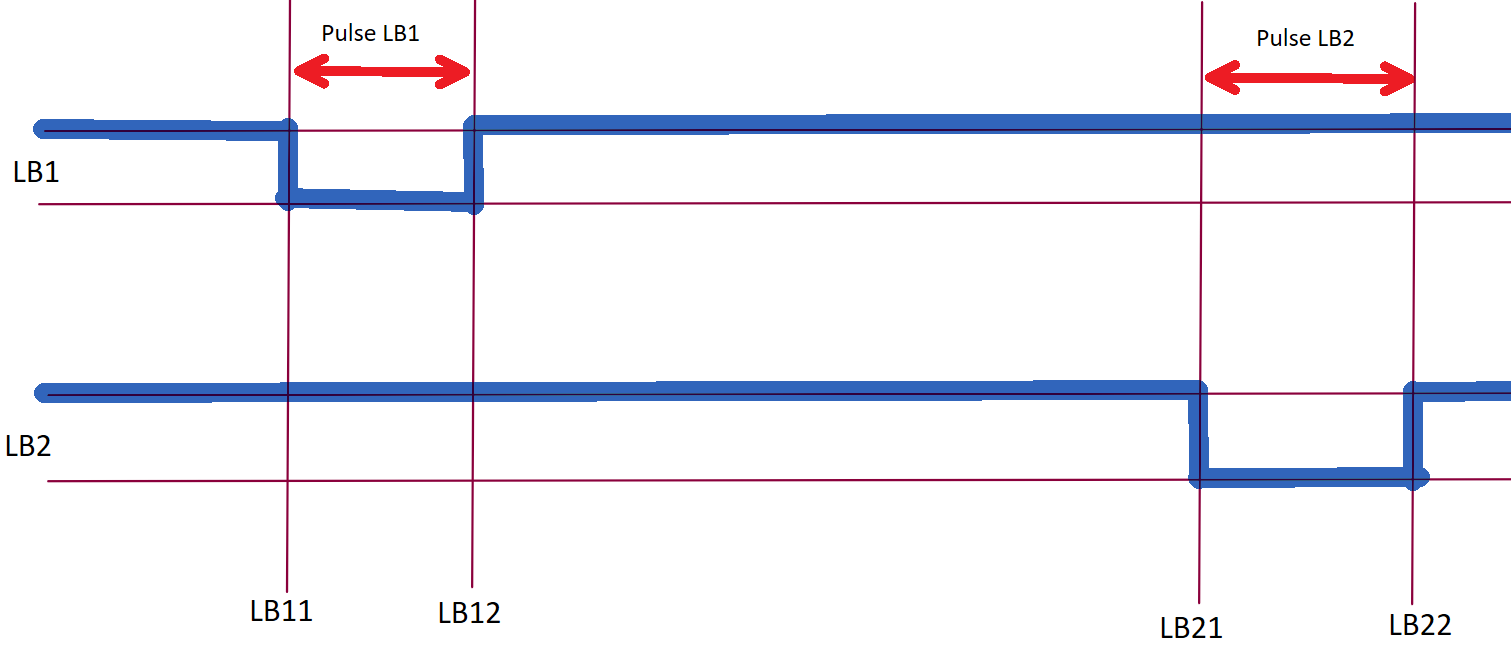
\includegraphics[width=\textwidth]{images/signals}
    \caption{Generierte Signale der Lichtschranke beim Durchflug eines Objekts abhängig der Zeit}
    \label{fig:ArdSigs}
\end{figure}


\clearpage
\subsection{Modi}
%\subsubsection{Preprocessor-Direktiven}
Mit\marg{Preprocessor} Hilfe der \#define Anweisung können 3 verschiedene Modis ausgewählt werden. Dafür müssen die entsprechenden Befehle ein-kommentiert werden.\\

\begin{tabular}{L{0.3\linewidth} L{0.6\linewidth}}
    \#define MYDEBUG & Aktiviert den Debuggmodus und somit die \textit{DEBUG\_PRINT}-Funktionen.\\
    \#define MYLOG & Aktiviert den Datenloggingmodus und somit die \textit{LOG\_PRINT}-Funktionen.\\
    \#define USEINTERRUPT & Aktiviert den Interruptmodus und deaktiviert den Pollingmodus.\\
\end{tabular}

\subsection{Globale Variabeln}
Es \marg{globale Variabeln} gibt folgende globale Variabeln:
\begin{itemize}
    \item const double sensordistance = 101.0*1000
    \item const double ballwidth = 72.0*1000
    \item unsigned long passingtime[4]
    \item double velocitykmh[4]
    \item int coubtingvar
\end{itemize}

\textit{sensordistance} und \textit{ballwidth} beschreiben die geometrischen Randbedingungen in $\mu m$.\\
\textit{passingtime} beinhaltet die Zeitstempel in $\mu s$ und \textit{velocitykmh} beinhlatet die gemessenen Geschwindigkeiten in $\nicefrac{km}{h}$.\\
Bei \textit{countigvar} handelt es sich um eine Lauf-variabel zur Indexierung der SerialPrint-Ausgaben.


\subsection{Hilfsfunktionen}
\subsubsection{calculate\_velocity\_ms()}\label{subsubsec:calcvel}
\begin{center}
    Geschwindigkeit [$\nicefrac{m}{s}$] = calculate\_velocity\_ms( Zeit [$\mu S$], Distanz [$\mu m$])
\end{center}

Die Funktion \textit{double calculate\_velocity\_ms(unsigned long passingduration,double distance)} übernimmt eine Zeitdauer in $\mu S$ und eine Distanz in $\mu m$.
Sie giebt eine Geschwindigkeit mit Hilfe der \ref{eq:Geschwindigkeit} in $\nicefrac{m}{s}$ zurück vom Typ double.\\


\subsubsection{printlog()}
Wenn der Datenloggingmodus aktiv ist printet die Funktion in die serielle Schnittstelle.
Im Pollingmodus:\\
\begin{tabular}{llll}
    Iteration&Bezeichnung& Puls LB1 & Puls LB2\\
\end{tabular}

Im Interruptmodus:\\
\begin{tabular}{llllll}
    Iteration&Bezeichnung& Int. LB1 & Int. LB2& Int. LB11 - LB21& Int. LB12 - LB22\\
\end{tabular}\\

\clearpage
\subsection{Polling-Modus}\label{subsec:polling}
Im \marg{Polling} Pollingmodus wird mit der Funktion \textit{\href{https://www.arduino.cc/reference/en/language/functions/advanced-io/pulsein/}{pulseIn(pin, value, timeout)}} die Länge des Unterbruches in $\mu S$ angegegeben. Die minimale dedektierbare Pulslänge ist dabei 10 $\mu S$.
Es werden folgende Zeiten erfasst und im Array \textit{passingtime} abgelegt:\\
\begin{tabular}{cll}
    \textbf{Index}&\textbf{Zeit [$\mu S$]} & \textbf{relevante Distanz} \\
    0&Pulse LB1 & Objektgrösse\\
    1&Pulse LB2 & Objektgrösse\\
\end{tabular}\\

Die Werte im Index 2 und 3 sind im Pollingmodus immer 0.\\

Mit der Funktion \textit{calculate\_velocity\_ms()}(Abschnitt \ref{subsubsec:calcvel}) kann die Geschwindigkeit in $\nicefrac{m}{s}$ berechnet werden. Danach wird das Resultat mit dem Faktor 3.6 multipliziert und im Array \textit{velocitykmh} abgelegt.\\

Die Werte im Index 2 und 3 sind im Pollingmodus immer 0.\\


\subsection{Interrupt-Modus} \label{subsec:interrupt}
Im \marg{Interrupt}Interruptmodus wird bei jedem Flankenwechsel ein Interrupt ausgelöst und ein Zeitstempel in $\mu S$ gespeichert.\\
\textbf{Beim Arduino UNO müssen die Lichtschranken dafür zwingend auf Pin 2 und 3 angeschlossen sein. Weiter muss zuerst die Lichtschranke 1 danach Lichtschranke 2 ausgelöst werden.}\\
Dies ergibt gesamt 4 Messwerte für LB11, LB12, LB21 und LB22 wie in \ref{fig:ArdSigs} gezeigt. Diese werden im Array \textit{passingtime} gespeichert.\\

Das Array \textit{passingtime} beinhaltet also im Interruptmodus die folgenden Einträge:\\
\begin{tabular}{cl}
    \textbf{Index}&\textbf{Zeit [$\mu S$]} \\
    0&LB11 \\
    1&LB12 \\
    2&LB21 \\
    3&LB22 \\
\end{tabular}\\

Mit der Funktion \textit{calculate\_velocity\_ms()}(\ref{subsubsec:calcvel}) kann die Geschwindigkeit in $\nicefrac{m}{s}$ berechnet werden. Danach wird das Resultat mit dem Faktor 3.6 multipliziert und im Array \textit{velocitykmh} abgelegt.\\

\begin{tabular}{cll}
    \textbf{Index}&\textbf{Zeit [$\mu S$]} & \textbf{relevante Distanz [$\mu m$]} \\
    0&LB12 - LB11 & Objektgrösse\\
    1&LB22 - LB21 & Objektgrösse\\
    2&LB21 - LB11 & Sensorabstand\\
    3&LB22 - LB12 & Sensorabstand\\
\end{tabular}\\

\subsubsection{Hilfsfunktionen}
Der Interruptmodus benötigt noch weitere Hilfsfunktionen, nämlich die Interrupt-Service-Routine. Weiter wird noch das Flag \marg{Interrupt-Flag} \textit{LBinterrupted} benötigt, welches auf True wechselt, sobald das Objekt den Punkt LB22 durchlaufen hat.

\paragraph{ISRLB1()}
Diese Funktion ist die Interrupt-Service-Routine für die Lichtschranke LB1. Sie erkennt den Signalwechsel und schreibt den aktuellen Zeitstempel LB11 oder LB12 je nach dem ob das Signal HIGH oder LOW ist. Weiter wird das Flag \textit{LBinterrupted} auf False gesetzt.\\


\paragraph{ISRLB2()}
Diese Funktion ist die Interrupt-Service-Routine für die Lichtschranke LB1. Sie erkennt den Signalwechsel und schreibt den aktuellen Zeitstempel LB11 oder LB12 je nach dem ob das Signal HIGH oder LOW ist. Bei LB21 wird das Flag \textit{LBinterrupted} auf False gesetzt. Bei LB22 auf True.\\

%
%Der \marg{Funktionen} Code besitzt folgende Funktionen:
%\begin{itemize}
%    \item void setup()
%    \item void loop()
%    \item double calculate\_velocity\_ms(unsigned long passingduration,double distance)
%    \item void printlog(double speedinkmh[4])
%    \item void ISRLB1()
%    \item void ISRLB2()
%\end{itemize}
%
%
%Das Array \textit{passingtime} beinhaltet die folgenden Einträge:\\
%\begin{tabular}{lll}
%    \textbf{Index}&\textbf{Zeit} & \textbf{Distanz} \\
%    0&LB12 - LB11 & Ballgrösse\\
%    1&LB22 - LB21 & Ballgrösse\\
%    2&LB21 - LB11 & Sensorabstand\\
%    3&B22 - LB12 & Sensorabstand\\
%\end{tabular}\\
%
%Das Array \textit{velocitykmh} beinhaltet die berechneten Geschwindigkeit korresponidrenden zu den Zeiten und Distanzen aus dem passingtime-Array.\\
%Im Pollingmodus sind die Werte bei  Index 2 und 3 jeweils 0.





\section{Python}
Das Pythonskript aus Anhang \ref{app:python} dient dazu, die gesendeten Daten über den Serialport auszulesen und in einem .txt File abzuspeichern. Dies erleichtert die Datenanalyse mit Excel oder Matlab. Eine direkte Auswertung in Phyton wäre ebenfalls möglich.\\

\subsection{Randbedingungen}
Die Baudrate im Python-Sktipt (Zeile 29) muss die selbe sein wie im Arduino-Code angegeben.\\
Der COM-Port sollte unter Windows automatisch gefunden werden. Ist dies nicht der Fall müssen die Zeilen 31 bis 38 angepasst werden. Das Argument \textit{serial\_port} kann dabei einfach mit dem gewünschten Port ersetzt werden.

\subsection{Messdaten}
Der Name des Ausgabefiles kann in Zeile 48 beliebig angepasst werden.

\subsection{Ablauf}
Wird das Skript gestartet erstellt es ein \*.txt-File und schreibt eine Kopfzeile.
Danach wird alle,s was über den gewählten Serialport empfangen wird in dieses .txt-File gespeichert.\\
Sobald ein KeyboardInterrupt erzeigt wird, beispielsweise mit Ctrl + C oder dem Abbruch-Knopf wird das File gespeichert und das Skript beendet.